%% Poster for JupyterCon
\documentclass{tikzposter}

\usepackage{geometry}
\geometry{
	papersize={90in, 44.5in},
}


\usepackage{lmodern}
\usepackage[fontsize=24pt]{scrextend}


% Recalculate page size
% https://tex.stackexchange.com/questions/220726/columns-environment-doesnt-scale-to-full-paper-size-tikzposter-using-custom-pa
\makeatletter
\setlength{\TP@visibletextwidth}{\textwidth-2\TP@innermargin}
\setlength{\TP@visibletextheight}{\textheight-2\TP@innermargin}
\makeatother

%% Tikzposter is highly customizable: please see
%% https://bitbucket.org/surmann/tikzposter/downloads/styleguide.pdf

%% Available themes: see also
%% https://bitbucket.org/surmann/tikzposter/downloads/themes.pdf
% \usetheme{Default}
% \usetheme{Rays}
\usetheme{Basic}
% \usetheme{Simple}
% \usetheme{Envelope}
% \usetheme{Wave}
% \usetheme{Board}
% \usetheme{Autumn}
% \usetheme{Desert}

%% Further changes to the title etc is possible
% \usetitlestyle{Default}
% \usetitlestyle{Basic}
% \usetitlestyle{Empty}
% \usetitlestyle{Filled}
% \usetitlestyle{Envelope}
% \usetitlestyle{Wave}
% \usetitlestyle{verticalShading}

%\usepackage{fontspec}
%\setmainfont{FreeSerif}
%\setsansfont{FreeSans}

\author{Matt Henderson, Oliver Evans, Shreyas Cholia, Fernando P\'{e}rez}
\title{Kale: Human-in-the-loop High Performance Computing with Jupyter}
\institute{Lawrence Berkeley National Laboratory}
%% Optional title graphic
%\titlegraphic{\includegraphics[width=7cm]{IMG_1934}}
%% Uncomment to switch off tikzposter footer
\tikzposterlatexaffectionproofoff

% arara: pdflatex
\begin{document}
\maketitle


\begin{columns}
\column{0.7}

\block{Overview} {
    \begin{itemize}
        \item We try to do this. What?
        \item we try to do that.
    \end{itemize}
}

\block{Scientific HPC Systems} {
    \begin{itemize}
        \item Optimized for machine efficiency
        \item Assumes automated workflows
        \item Post-mortem analyses
    \end{itemize}
}

\block{Scientific Workflows Operated by Humans} {
    \begin{itemize}
        \item Manual inspection
        \item Manual intervention
        \item Experimentation and Dynamic updates during execution
    \end{itemize}
}

\block{Jupyter Interactive HPC} {
    \begin{itemize}
        \item Realtime Dashboards and Widgets
        \begin{itemize}
            \item Batch Queues
            \item Workflow status
            \item Task resource use
            \item Task file output
        \end{itemize}
        \item Workflow Control Center
        \begin{itemize}
            \item Build
            \item Control
            \item Interact
        \end{itemize}
    \end{itemize}
}    

\block{Development Environment} {
    \begin{itemize}
        \item Development Environment
        \item Remote kernels
        \item Resource details for debugging
    \end{itemize}
}


\column{0.3}

\block{Screenshot}{%
This screenshot has nothing to do with our project.
\begin{tikzfigure}[Figures in tikzposter]
    Test \\
    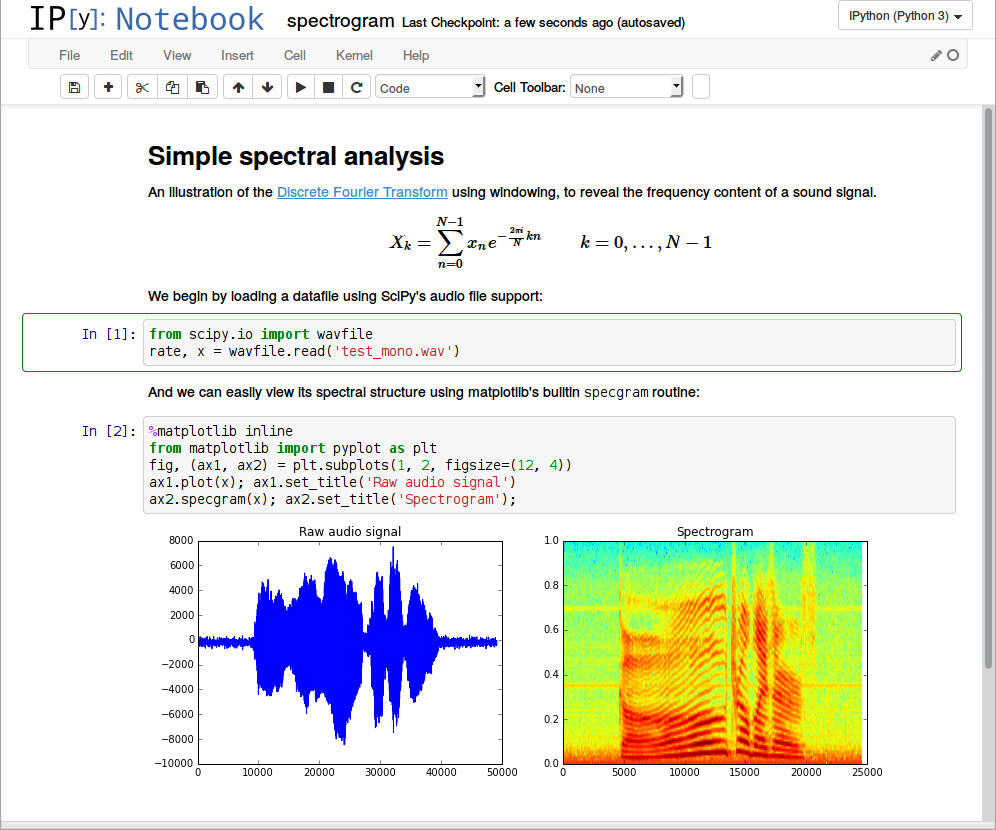
\includegraphics[width=\linewidth]{example-notebook}
\end{tikzfigure}
}

\end{columns}


\end{document}
